\chapter{Appendix}

\section{Datasets}

%TODO: Change title in figure
\begin{figure}[ht]
	\centering
	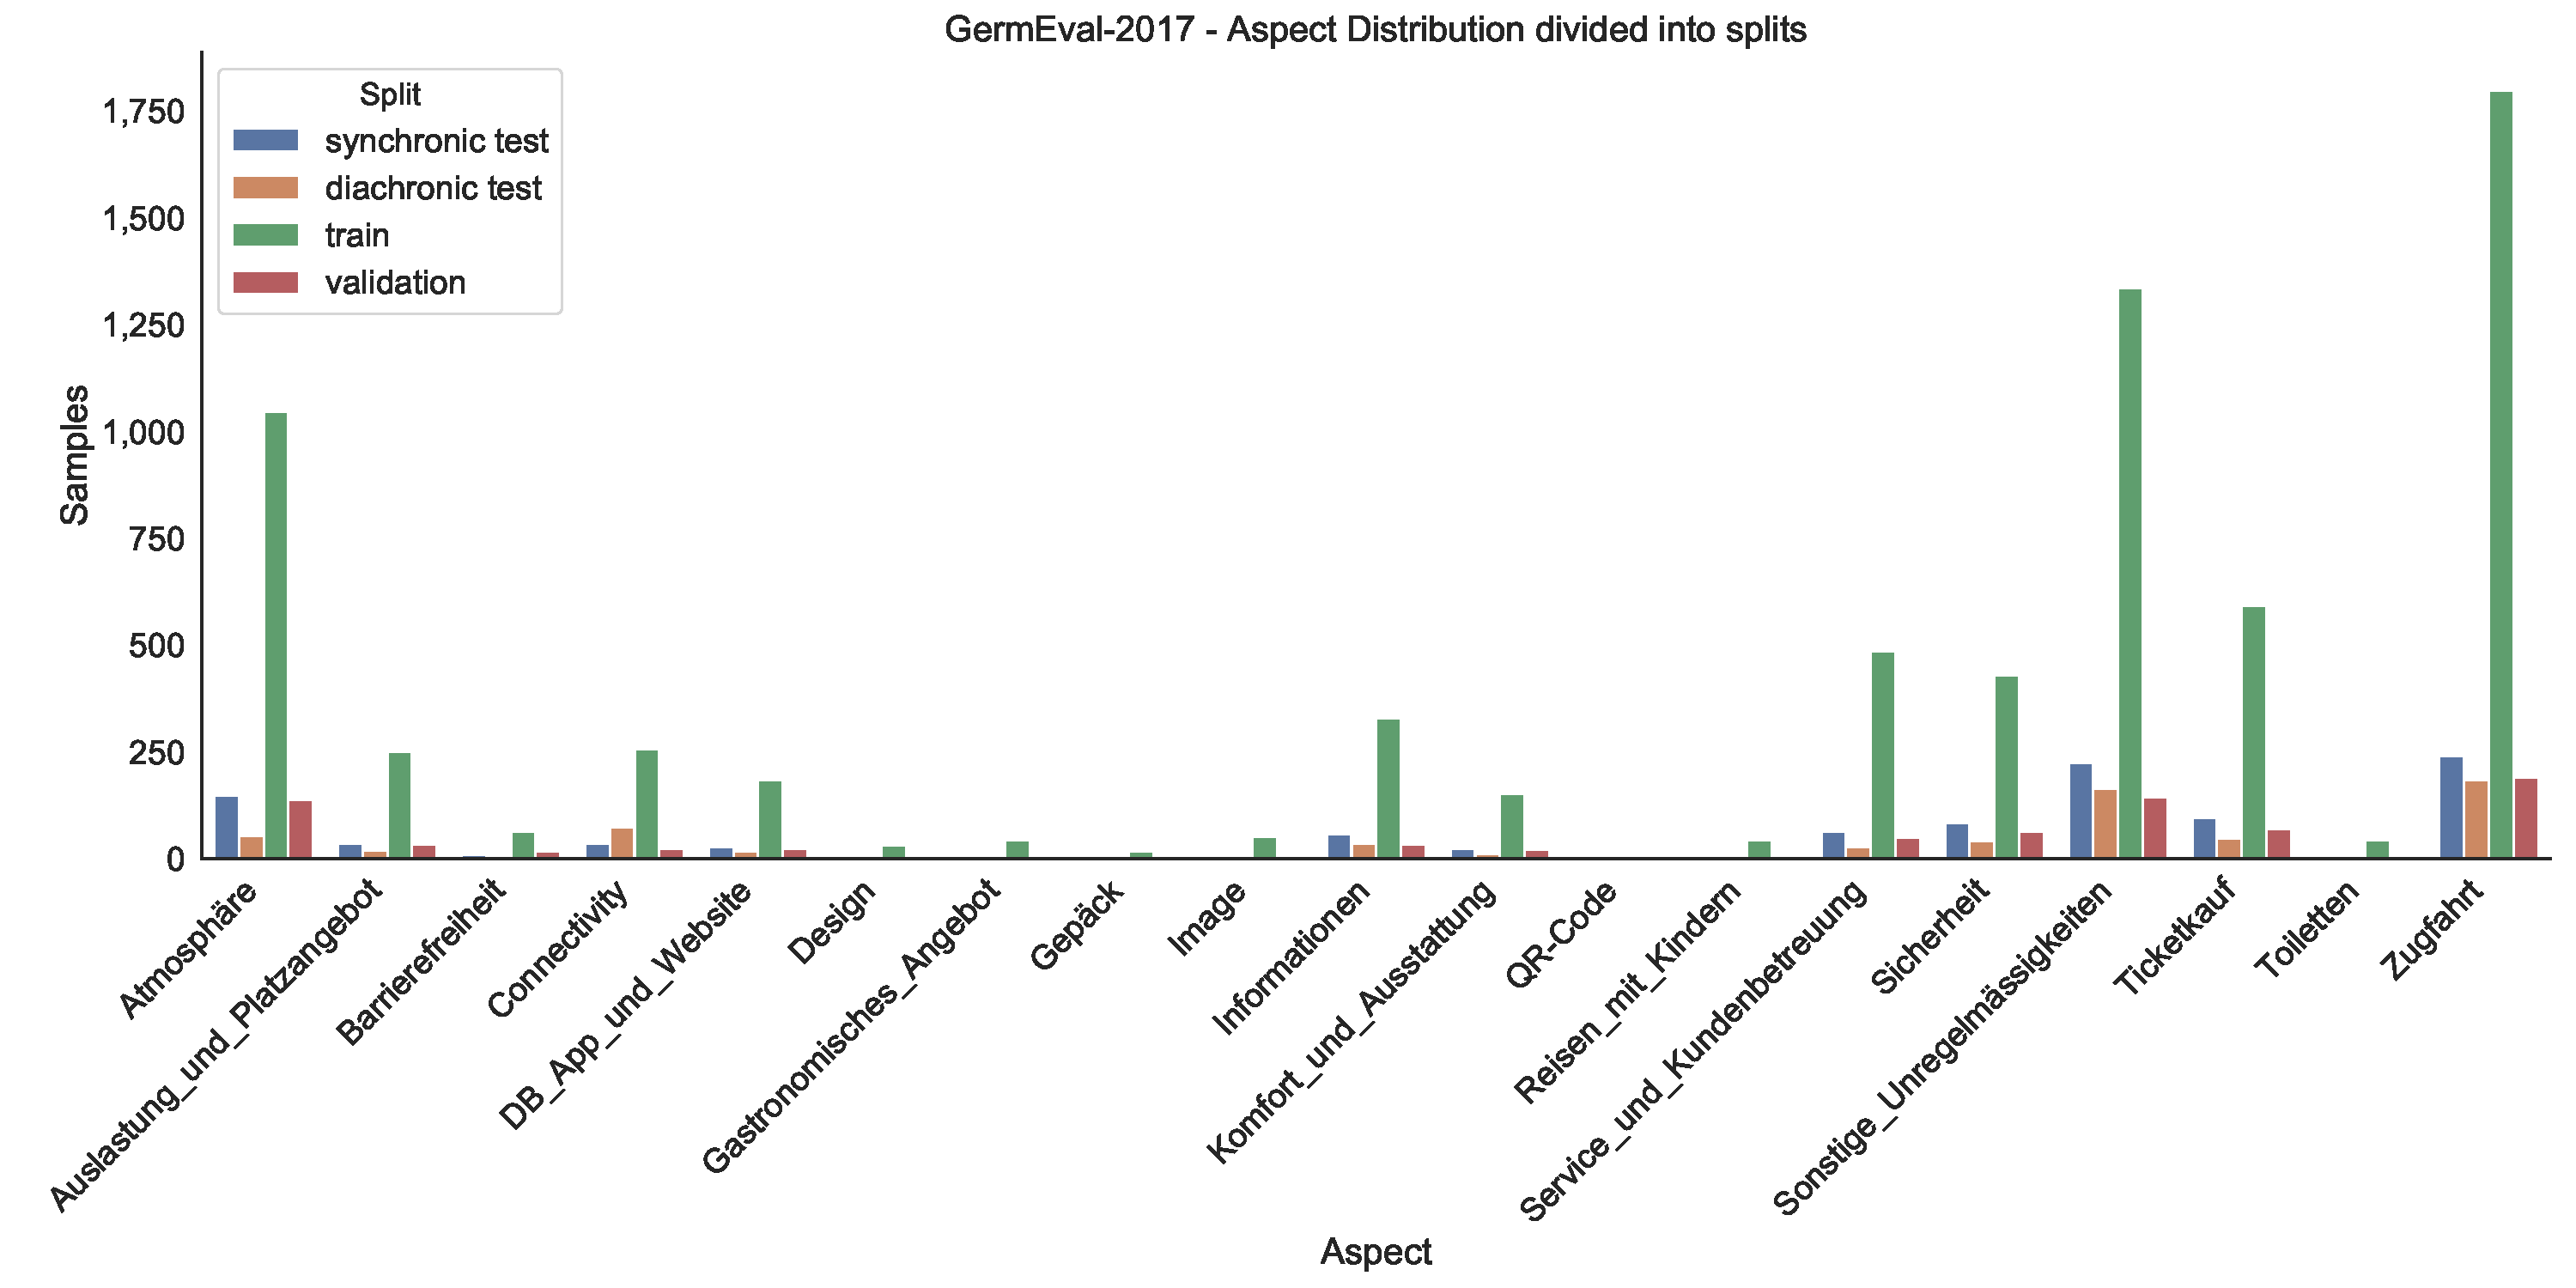
\includegraphics[width=\textwidth]{figures/08_appendix/08_germevalAspects}
	\caption{Statistics on GermEval-2017 aspects}
	\label{fig:08_germEvalStatistics}
\end{figure}


\begin{figure}[ht]
	\centering
	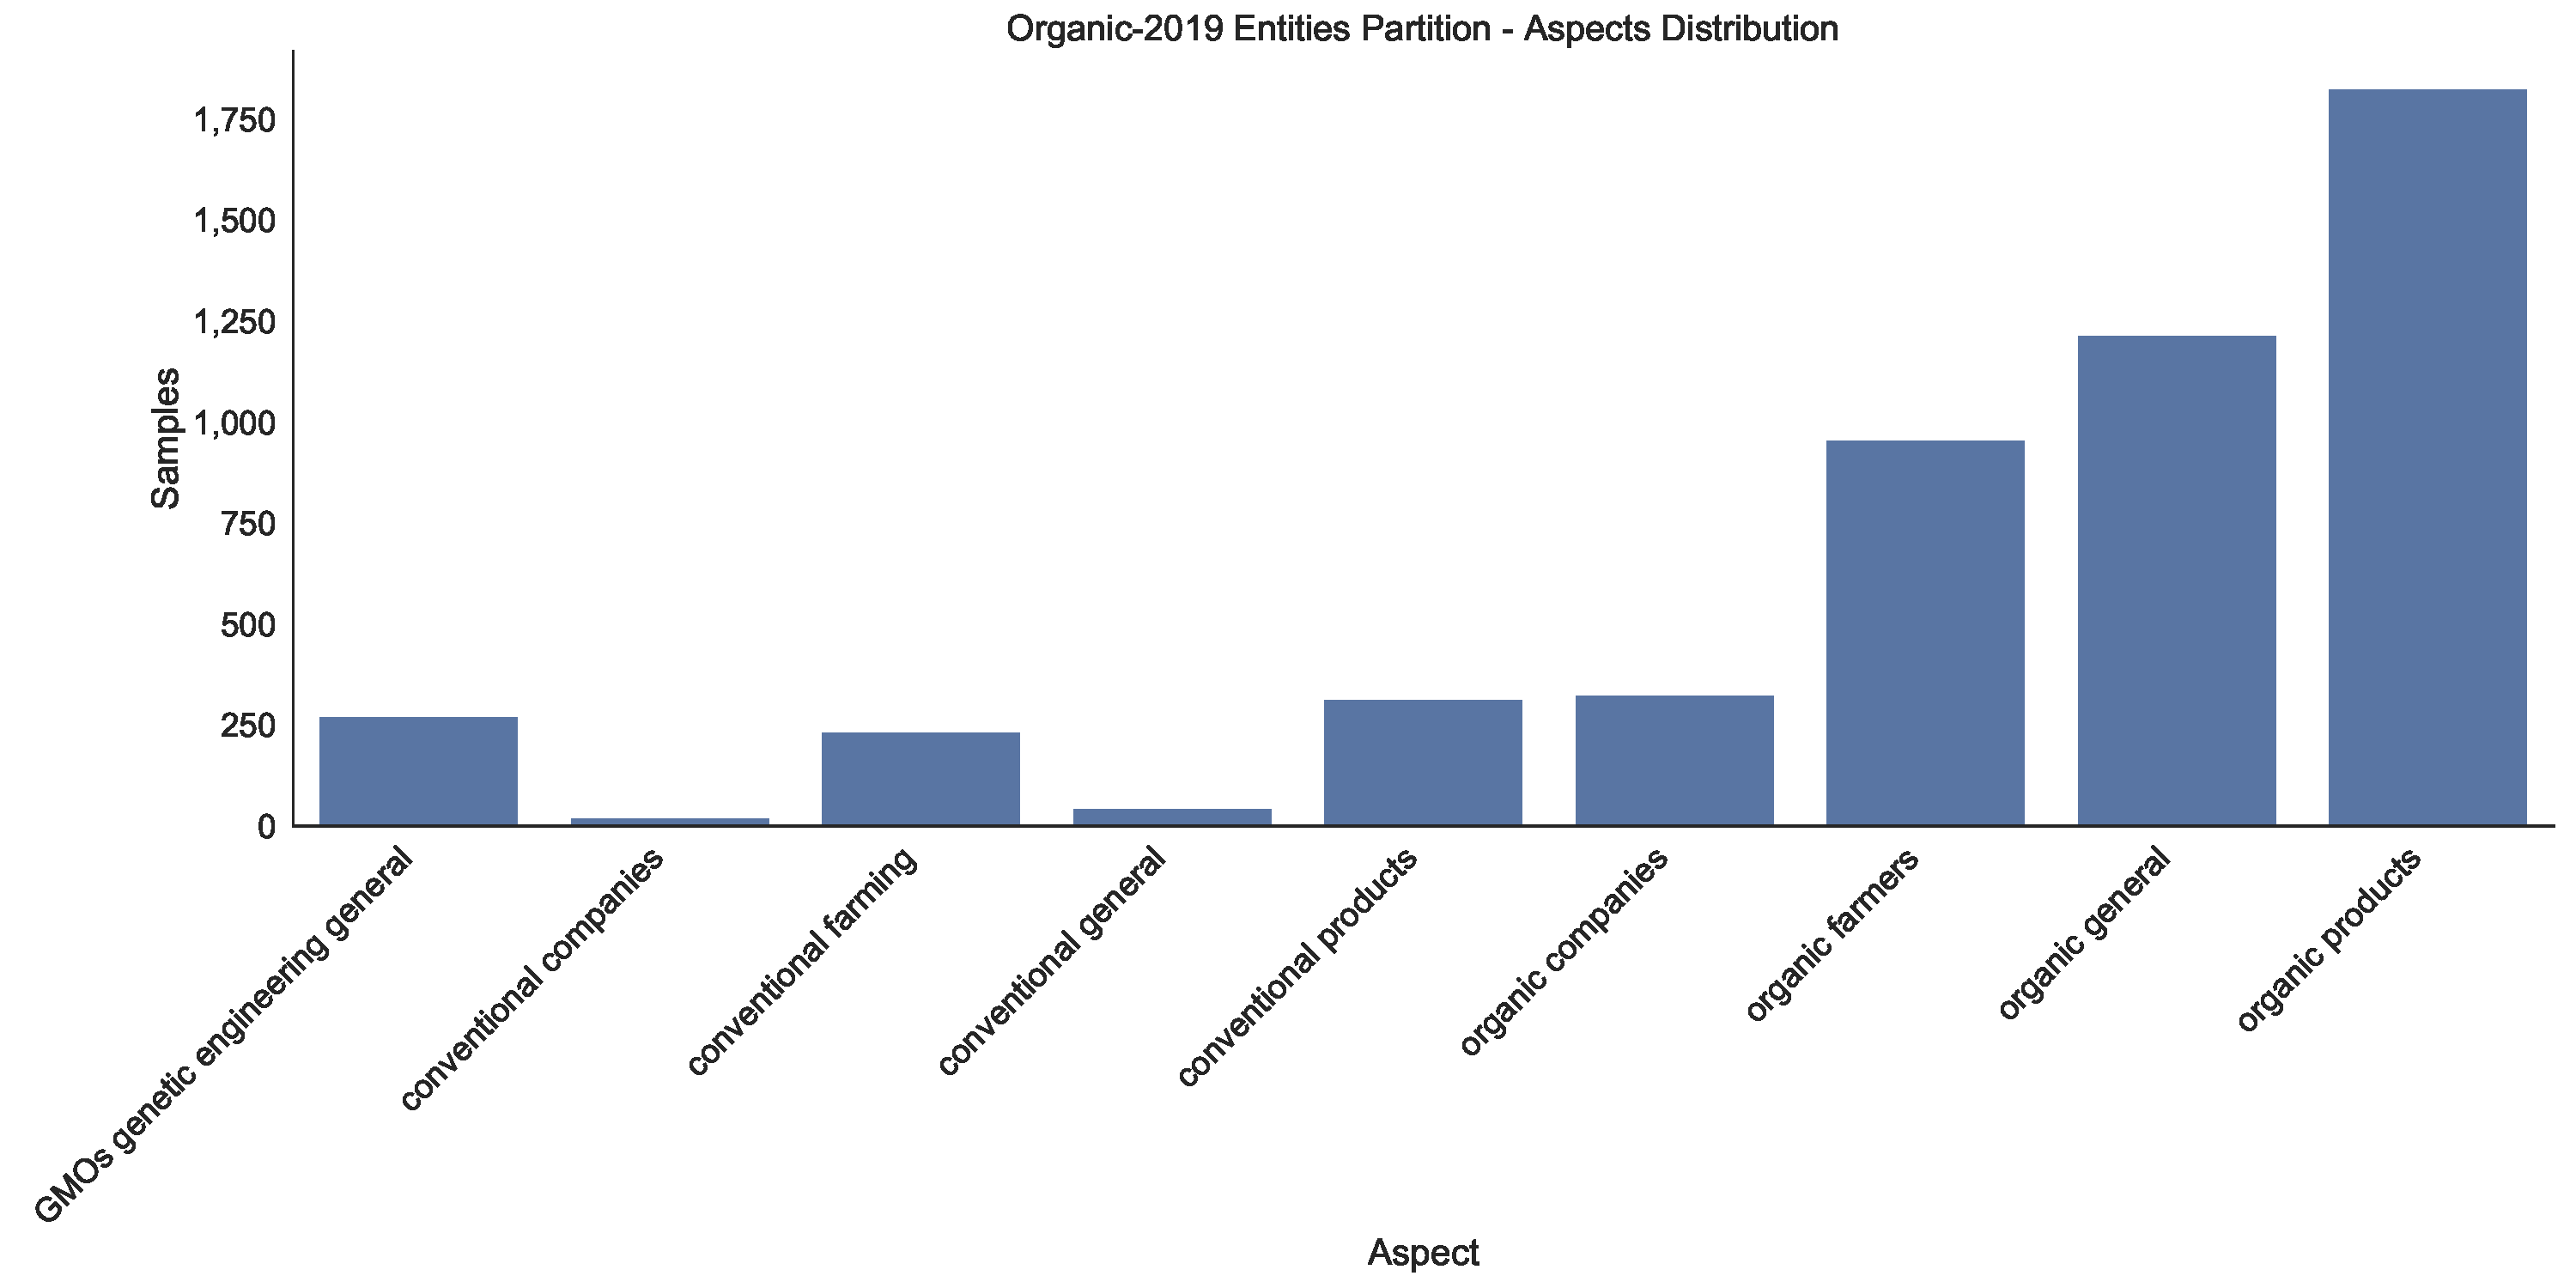
\includegraphics[width=\textwidth]{figures/05_setup/05_organicEntities}

	\caption{Distribution of the aspect \textit{entity} in the Organic-2019 dataset.}
	\label{fig:05_organic2019_Entities}
\end{figure}

\begin{figure}[ht]
	\centering
	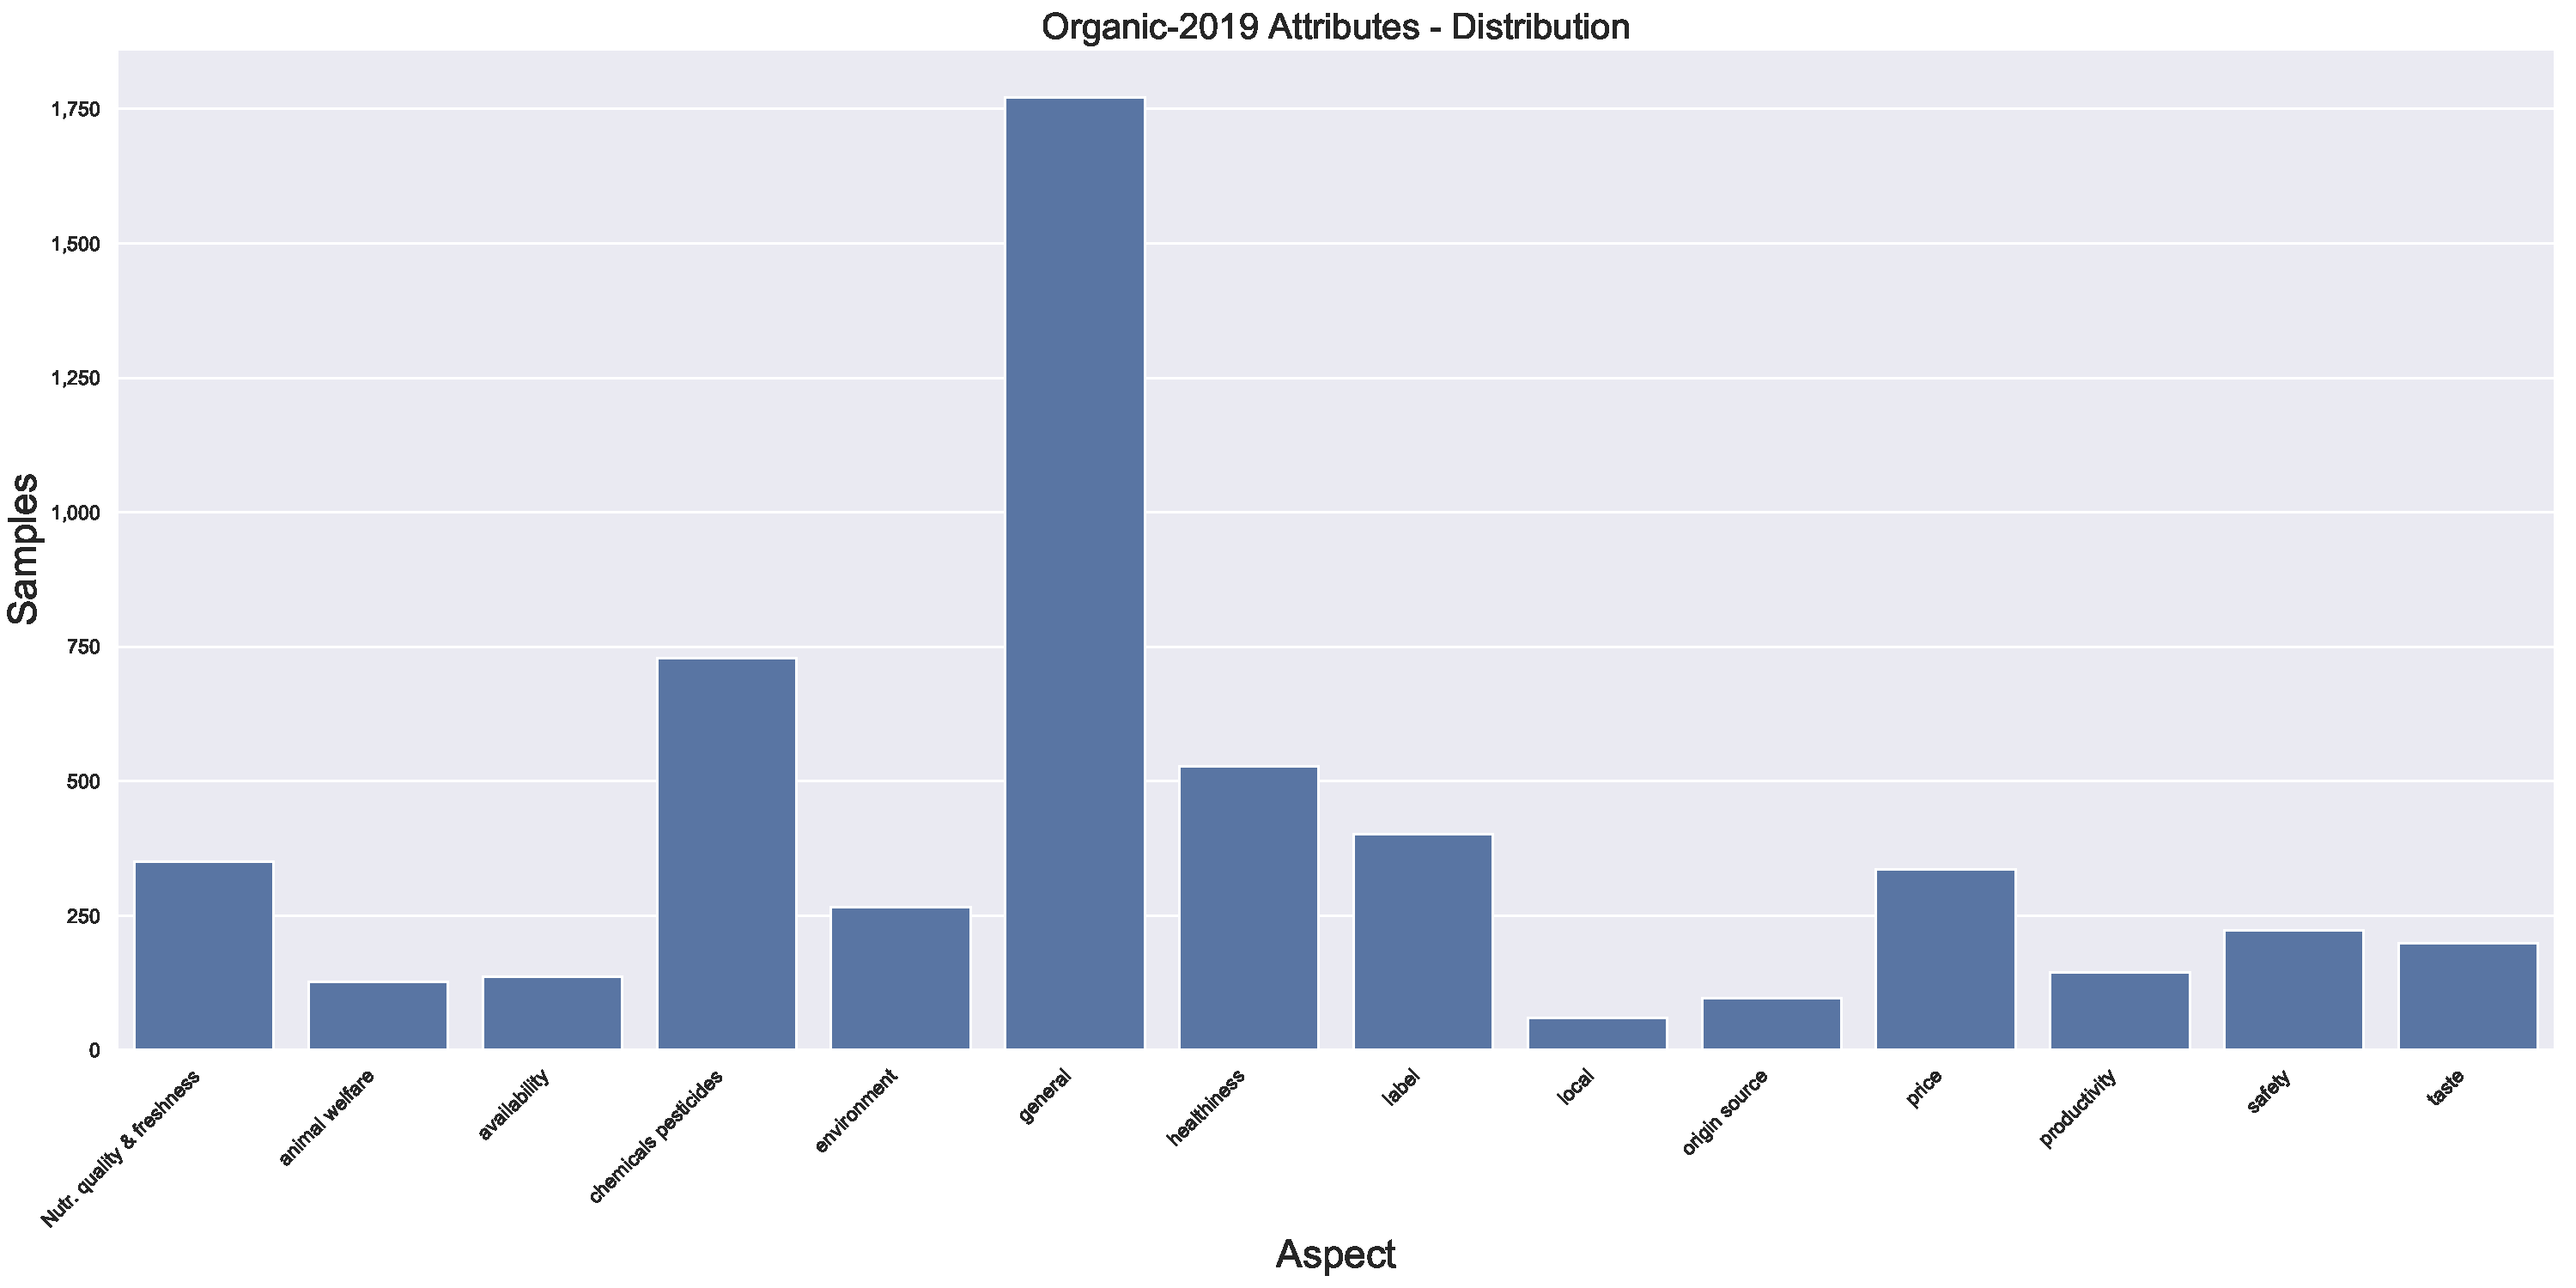
\includegraphics[width=\textwidth]{figures/05_setup/05_organicAttributes}
	\caption{Distribution of the aspect \textit{attribute} in the Organic-2019 dataset.}
	\label{fig:05_organic2019_Attributes}
\end{figure}

	

\section{Optimization}

\begin{table}
	\begin{center}
		\begin{tabular}{lclc}
		\toprule
		\multicolumn{4}{c}{OLS regression for Validation Loss / HyperOpt Iterations} \\
		\midrule
		\textbf{Dep. Variable:}    &        y        & \textbf{  R-squared:         } &     0.009   \\
		\textbf{Model:}            &       OLS       & \textbf{  Adj. R-squared:    } &    -0.002   \\
		\textbf{Method:}           &  Least Squares  & \textbf{  F-statistic:       } &    0.8307   \\
		\textbf{Date:}             & Mi, 24 Apr 2019 & \textbf{  Prob (F-statistic):} &    0.365    \\
		\textbf{Time:}             &     15:32:34    & \textbf{  Log-Likelihood:    } &   -51.223   \\
		\textbf{No. Observations:} &          90     & \textbf{  AIC:               } &     106.4   \\
		\textbf{Df Residuals:}     &          88     & \textbf{  BIC:               } &     111.4   \\
		\textbf{Df Model:}         &           1     & \textbf{                     } &             \\
		\bottomrule
		\end{tabular}
		\begin{tabular}{lcccccc}
					   & \textbf{coef} & \textbf{std err} & \textbf{t} & \textbf{P$>$$|$t$|$} & \textbf{[0.025} & \textbf{0.975]}  \\
		\midrule
		\textbf{const} &       0.3598  &        0.090     &     3.980  &         0.000        &        0.180    &        0.539     \\
		\textbf{x1}    &      -0.0016  &        0.002     &    -0.911  &         0.365        &       -0.005    &        0.002     \\
		\bottomrule
		\end{tabular}
		\begin{tabular}{lclc}
		\textbf{Omnibus:}       & 163.475 & \textbf{  Durbin-Watson:     } &     2.062  \\
		\textbf{Prob(Omnibus):} &   0.000 & \textbf{  Jarque-Bera (JB):  } & 11634.826  \\
		\textbf{Skew:}          &   6.940 & \textbf{  Prob(JB):          } &      0.00  \\
		\textbf{Kurtosis:}      &  56.944 & \textbf{  Cond. No.          } &      102.  \\
		\bottomrule
		\end{tabular}
	\end{center}
	\caption{\gls{ols} Regression statistics for a regression of HyperOpt \gls{tpe} optimization losses on the validation set {(Dataset: GermEval-2017)}}
	\label{tab:08_olsLossItVal}	
\end{table}

\begin{table}
	\begin{center}
		\begin{tabular}{lclc}
		\toprule
		\multicolumn{4}{c}{OLS regression for Test Loss / HyperOpt Iterations} \\
		\midrule
		\textbf{Dep. Variable:}    &        y        & \textbf{  R-squared:         } &     0.006   \\
		\textbf{Model:}            &       OLS       & \textbf{  Adj. R-squared:    } &    -0.006   \\
		\textbf{Method:}           &  Least Squares  & \textbf{  F-statistic:       } &    0.4930   \\
		\textbf{Date:}             & Mi, 24 Apr 2019 & \textbf{  Prob (F-statistic):} &    0.484    \\
		\textbf{Time:}             &     16:22:21    & \textbf{  Log-Likelihood:    } &   -206.16   \\
		\textbf{No. Observations:} &          90     & \textbf{  AIC:               } &     416.3   \\
		\textbf{Df Residuals:}     &          88     & \textbf{  BIC:               } &     421.3   \\
		\textbf{Df Model:}         &           1     & \textbf{                     } &             \\
		\bottomrule
		\end{tabular}
		\begin{tabular}{lcccccc}
					& \textbf{coef} & \textbf{std err} & \textbf{t} & \textbf{P$>$$|$t$|$} & \textbf{[0.025} & \textbf{0.975]}  \\
		\midrule
		\textbf{const} &       0.8356  &        0.506     &     1.653  &         0.102        &       -0.169    &        1.840     \\
		\textbf{x1}    &      -0.0069  &        0.010     &    -0.702  &         0.484        &       -0.026    &        0.013     \\
		\bottomrule
		\end{tabular}
		\begin{tabular}{lclc}
		\textbf{Omnibus:}       & 191.171 & \textbf{  Durbin-Watson:     } &     2.030  \\
		\textbf{Prob(Omnibus):} &   0.000 & \textbf{  Jarque-Bera (JB):  } & 25929.119  \\
		\textbf{Skew:}          &   9.027 & \textbf{  Prob(JB):          } &      0.00  \\
		\textbf{Kurtosis:}      &  84.169 & \textbf{  Cond. No.          } &      102.  \\
		\bottomrule
		\end{tabular}
	\end{center}
	\caption{\gls{ols} Regression statistics for a regression of HyperOpt \gls{tpe} optimization losses on the test set {(Dataset: GermEval-2017)}}
	\label{tab:08_olsLossItTest}	
\end{table}

\begin{table}[]
	\centering
	\begin{tabular}{@{}lll@{}}
	\toprule
	Variable           & Type       & Parameters                \\ \midrule
	Batch Size         & QUniform   & Interval: {[}1, 100{]}    \\
	Comment Clipping   & QUniform   & Interval: {[}10, 250{]}   \\
	Replace URL Tokens & Bool       & {[}True, False{]}         \\
	Use Stop Words     & Bool       & {[}True, False{]}         \\
	Use Spell Checker  & Bool       & {[}True, False{]}         \\
	Harmonize Bahn     & Bool       & {[}True, False{]}         \\
	Embedding Type     & Choice     & {[}Glove, Fasttext{]}     \\
	\# Encoder Blocks  & QUniform   & Interval {[}1, 8{]}       \\
	\# Attention Heads & Choice     & {[}1, 2, 3, 4, 5{]}       \\
	PW Layer Size      & QUniform   & Interval: {[}32, 256{]}   \\
	TF Dropout         & Uniform    & Interval {[}0, 0.8{]}     \\
	Output Dropout     & Uniform    & Interval {[}0, 0.8{]}     \\
	Transformer Bias   & Bool       & {[}True, False{]}         \\
	LR Warmup          & QUniform   & Interval {[}1000, 9000{]} \\
	LR Factor          & Uniform    & Interval {[}0.01, 4{]}    \\
	Adam $\beta 1$        & Uniform    & Interval {[}0.7, 0.999{]} \\
	Adam $\beta 2$        & Uniform    & Interval {[}0.7, 0.999{]} \\
	Adam EPS           & LogUniform & log(1e-10), log(1)        \\
	LR                 & LogNormal  & log(0.01, log(10)         \\
	Weight Decay       & QUniform   & $1e^{[-8, -3]}$       \\
	Output Layer       & Choice     & {[}CNN*, LinSum{]}        \\
	\# CNN Filter*     & QUniform   & Interval {[}1, 400{]}     \\
	Kernel Size*       & QUniform   & Interval {[}1, 10{]}      \\
	Stride*            & QUniform   & Interval {[}1, 10{]}      \\
	Padding*           & QUniform   & Interval {[}0, 5{]}       \\ \bottomrule
	\end{tabular}
	\caption{Hyperparameter Search space for GermEval-2017. * marks parameters which are only sampled if CNN is chosen as the output layer.}
	\label{tab:08_hpSpace}	
\end{table}

\begin{figure}[ht]
	\centering
	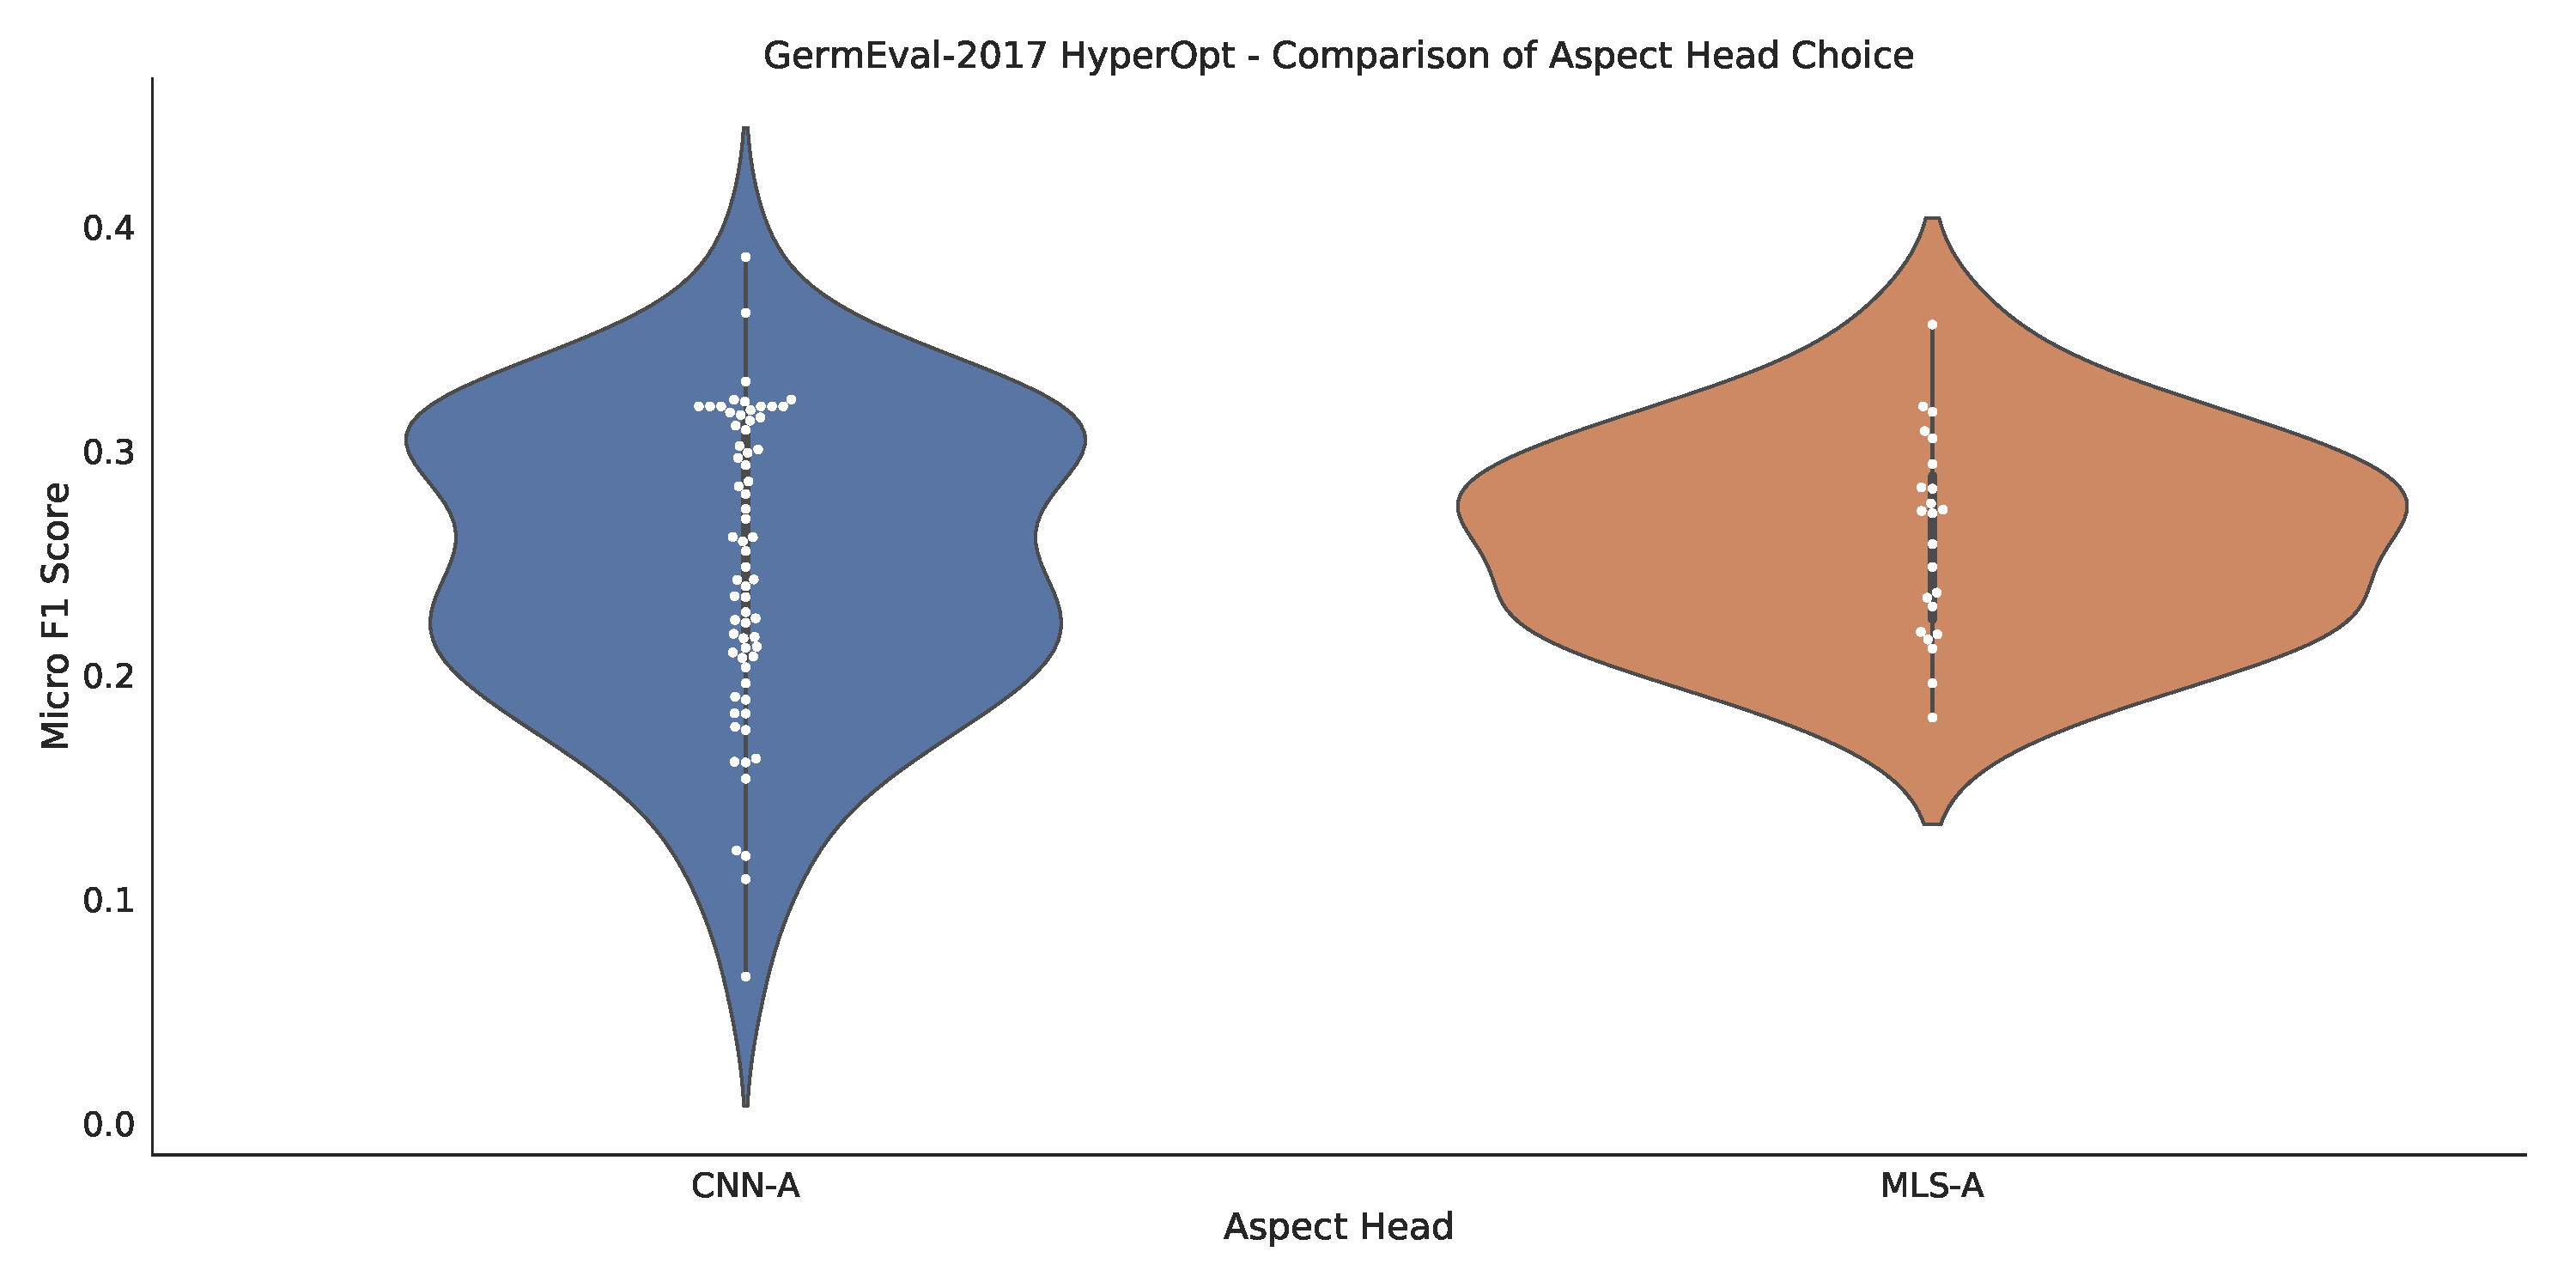
\includegraphics[width=\textwidth]{figures/06_results/06_hp_ge_vio_aspectHead_test}
	\caption{Hyperopt - Comparison and impact of aspect head choices and sampling amount}
	\label{fig:06_ge_aspectHeadChoices}
\end{figure}
